%==============================================================================
% Voorbeeld hogent-article: onderzoeksvoorstel bachproef
%==============================================================================

\documentclass{hogent-article}

\usepackage{lipsum} % Voor vultekst
\usepackage{bytefield} % Voor TCP Header
\usepackage{graphicx} % Voor grafiek TCP Equilibrium
\graphicspath{ {./img/} }

% Invoegen bibliografiebestand
\addbibresource{references.bib}

% Informatie over de opleiding, het vak en soort opdracht
\studyprogramme{Professionele bachelor toegepaste informatica}
\course{Bachelorproef}
\assignmenttype{Paper: Onderzoeksvoorstel}
\academicyear{2023-2024}


\title{Scripting voor Netwerkoptimalisatie: DNS- en DHCP-Beheer met Python-scripts en IP Address Management Integratie}
\author{Stijn Coppens}
\email{stijn.coppens@student.hogent.be}

\projectrepo{https://github.com/stcoppens/Bachelorproef}

% Binnen welke specialisatierichting uit 3TI situeert dit onderzoek zich?
% Kies uit deze lijst:
%
% - Mobile \& Enterprise development
% - AI \& Data Engineering
% - Functional \& Business Analysis
% - System \& Network Administrator
% - Mainframe Expert
% - Als het onderzoek niet past binnen een van deze domeinen specifieer je deze
%   zelf
%
\specialisation{System \& Network Administrator}
% Geef hier enkele sleutelwoorden die je onderwerp beschrijven
\keywords{DNS, DHCP, IPAM, Python}

\begin{document}

\begin{abstract}
Netwerkconfiguraties worden momenteel grotendeels handmatig beheerd, wat inefficiënt is als proces, en tevens gevoelig is voor menselijke fouten. Het minimaliseren van handmatig beheer van netwerkconfiguraties zou leiden tot efficiëntiewinsten, tijdswinsten en verminderde complexiteit.
Deze bachelorproef richt zich op het ontwikkelen van een innovatieve, geautomatiseerde benadering voor netwerkbeheer (en IP-adresallocatie), door
middel van Python-scripts.
Het hoofddoel is het creëren van een abstractielaag boven een bestaande netwerkbeheertool voor DNS en DHCP,
waarbij de API van een IP Address Management (IPAM)-tool wordt aangestuurd. Deze abstractielaag maakt interactie met de IPAM-tool mogelijk via Python-scripts en wordt toegepast door API-aanroepen vanuit een intuïtief webportaal.
\end{abstract}
\tableofcontents

\bigskip

\section{Inleiding}%
\label{sec:inleiding}
In de hedendaagse technologische omgeving is netwerkbeheer van cruciaal belang voor de \\soepele werking van bedrijfsinfrastructuren. 
\\ Traditioneel vereist het beheren van \\netwerkconfiguraties, met name \textit{Domain Name System (DNS)} en \textit{Dynamic Host Configuration Protocol (DHCP)}, een grote mate van handmatige inspanning. Dat kan leiden tot inefficiëntie en menselijke fouten. 
Om dit op te lossen bestaan er meerdere \textit{Internet Protocol Address Management (IPAM)} softwarepakketten om de taken van netwerkbeheerders te automatiseren. 

% Het hoofddoel van deze bachelorproef is het ontwikkelen van een praktische oplossing voor netwerkbeheer door middel van python-scripts, waardoor een abstractielaag bovenop een IPAM-tool ontstaat. Deze laag zal de interactie mogelijk maken tussen een webportaal waar gebruikers veel voorkomende acties kunnen aanvragen die dan mits goedkeuring van de netwerkberheerder de IPAM kunnen aansturen.

Dit onderzoek zal een antwoord bieden op de vraag hoe je via python scripts een abstractielaag kan voorzien om via een webapplicatie veelgebruikte acties door te sturen naar de \textit{Application Programming Interface (API)} van een IPAM-tool. 

Uit dit project worden volgende voordelen verwacht:
\begin{itemize}
    \item Verminderde complexiteit voor \\veelgebruikte acties zoals het reserveren van IP-adressen.
    \item Tijdwinst door het uitsluiten van handmatig beheer.
    \item Efficiëntie door het vermijden van menselijke fouten.
    \item Verbetering van gebruiksvriendelijkheid
\end{itemize}
Deze voordelen zullen dragen bij aan een gestroomlijnde netwerkinfrastructuur.

% Dit onderzoek zal een eerste versie van het webportaal maken waarop gebruikers een \textit{Internet Protocol (IP)} reservatie kunnen aanvragen, wijzigen of verwijderen, nadat deze actie is goedgekeurd door een netwerkbeheerder zal deze dan uitgevoegd worden door de IPAM.

% TODO: (fase 1) introduceer je gekozen onderwerp, formuleer de onderzoeksvraag en deelvragen. Wat is de doelstelling (is die S.M.A.R.T.?), wat zal het resultaat zijn van het onderzoek (een Proof-of-Concept, een prototype, een advies, ...)? Waarom is het nuttig om dit onderwerp te onderzoeken?

\section{Begrippen}
\label{sec:begrippen}
Internet Protocol (IP) is het fundament van elk gestructureerd, goed functionerend en veilig netwerk. Het geeft de mogelijkheid efficiënt gegevens te routeren, netwerken te verdelen in meer beheersbare eenheden, toegang te beperken tot gevoelige data of systemen, services te identificeren en het oplossen van netwerkproblemen \autocite{Postel1981}. Dit hoofdstuk legt uit wat DNS en DHCP is en waarom IPAM helpt bij het beheren van IP netwerken. 

\subsection{DNS}
\textcite{Mockapetris1987} schrijft dat DNS een systeem is dat \textit{resource records} gebruikt om onder andere vertalingen te voorzien tussen domeinnamen en IP-adressen. Als voorbeeld kan je via de browser naar google surfen via het IP-adres \textit{142.251.36.35} of via het domeinnaam\\ \textit{www.google.be}.
\\ \\
Zoals beschreven door \textcite{Mockapetris1987} voorziet DNS meerdere types resource records die netwerkbeheerders kunnen meegeven: 
\begin{itemize}
    \item \textbf{A}: Dit resource record beschrijft een host adres. 
    Vb. \textit{”server1.voorbeeld.com IN A \\192.168.1.1”} maakt de vertaling zodat het toestel met de domeinnaam \textit{server1.voorbeeld.com} bereikbaar is zowel via het IP-adres \textit{192.168.1.1} als via de domeinnaam. 
    \item \textbf{CNAME}: Dit resource record beschrijft de kanonieke naam van een host, het wordt gebruikt om een alias of subdomein naar het hoofddomein door te verwijzen. Vb.\\ \textit{"www.voorbeeld.com. IN CNAME \\server1.voorbeeld.com"} zorgt dat server1 ook bereikbaar is via "\textit{www.voorbeeld.com}".
    \item \textbf{MX}: Dit resource record is een \textit{mail exchange} record en wordt gebruikt om aan te geven welke mailservers verantwoordelijk zijn voor het ontvangen van mails binnen een domein. vb. \textit{"voorbeeld.com. IN MX 10 mailserver.voorbeeld.com"} geeft de DNS server mee welke server de mailserver is.
    \item \textbf{NS}: Dit resource record is een \textit{name server} record, het beschrijft welke DNS-servers verantwoordelijk zijn voor het beheren van DNS-informatie voor een domein. Vb. \textit{"voorbeeld.com IN NS dns1.voorbeeld.com"} verwijst naar \textit{dns1} als DNS-server voor het domein “\textit{voorbeeld.com}”.
    \item \textbf{PTR}: Dit resource record is een \textit{Pointer} record, het wordt gebruikt om via IP een vertaling te vragen aan de DNS-server in plaats van via de naam.
    \item \textbf{SOA}: Dit resource record is een \textit{Start of Authority} record die belangrijke informatie bevat over de zone, zoals welke de primaire DNS-server, contactpersonen, etc.
\end{itemize}

\subsection{DHCP}
Dit protocol voorziet een framework voor het doorgeven van configuratie informatie naar \\hosts (lees: computers) op het netwerk . Zo kan een computer bijvoorbeeld een IP-adres ontvangen waarmee die kan communiceren binnen het netwerk waarop die is aangesloten \autocite{Droms1997}.

IP-netwerken worden door netwerkbeheerders op een logische manier opgesplitst in subnetwerken. Hierbij worden de beschikbare IP-adressen verdeeld in subnetwerken (subnet). Toestellen binnen subnet A zullen elkaar kunnen bereiken terwijl een toestel in een subnet B zonder de nodige routering geen verbinding zal kunnen maken met de toestellen in subnet A.

Voor DHCP zullen netwerkbeheerders subnets (of pools van IP-adressen) aanbieden aan de DHCP-server. Die zal gebruik maken van deze pools door (onder andere) IP-adressen uit te delen aan toestellen die verbinden op het netwerk en daarbij de DHCP-server laten weten dat ze nog geen IP-adres hebben.

\textcite{Droms1997} schrijft dat DHCP drie mechanismes gebruikt voor het uitdelen van IP-adressen:
\begin{itemize}
    \item \textbf{Automatisch}: Permanent toewijzen van een IP-adres.
    \item \textbf{Dynamisch}: IP-adres voor een bepaalde tijd toewijzen.
    \item \textbf{Manueel}: Een (door de netwerkbeheerder) vooraf bepaald IP-adres toewijzen, in vakjargon noemt met dit een IP-reservatie.
\end{itemize}

\subsection{IPAM}
Naast de vele uitdagingen die zowel DNS als DHCP met zich meebrengen, is het beheren van de vele DNS records, IP-adres ranges en de vaak vele IP-reservaties zeker iets waar een netwerkbeheerder over moet waken. 
Een mogelijke oplossing hiervoor is het gebruiken van IP Address Management (IPAM) via softwarepakketten die IPAM aanbieden.
IPAM laat toe IP-adressen efficiënt te beheren in een netwerk, het leidt tot een gestructureerde aanpak waardoor conflicten tussen subnetten worden vermeden. Het geeft een compleet overzicht van het netwerk met percentages van hoeveel adressen beschikbaar en in gebruik zijn. IPAM geeft eveneens de mogelijkheid om de historiek bij te houden waardoor het van pas komt voor schaalbaarheid en beveiliging van het netwerk \autocite{Rooney2020}.

\section{Probleemstelling}
\label{sec:probleemstelling}
Deze bachelorproef zal uitgevoerd worden bij Universiteit Gent (UGent), dienst ICT. Momenteel werkt UGent met scripts die op basis van zo genaamde subnetbestanden de nodige acties uitvoeren op de DHCP en DNS servers. 

Deze subnetbestanden stellen elk een subnet voor en beschrijven cruciale informatie zoals DNS-servers, welk \textit{Virtual Local Area Network (VLAN)} nummer, gateway, etc. Hiernaast bevatten deze zowel alle beschikbare als gereserveerde IP-adressen met daarbij eventueel enkele regels voor DNS en beveiliging.

Voor elke IP reservatie die moet gebeuren, \\krijgt het netwerkteam via een webportaal van intern UGent-personeel een mail met daarin de nodige hostinformatie die ze in het daarvoor bestemde subnetbestand plakken. Indien hier nog extra DNS- of beveiligingsregels bij horen, moet de netwerkbeheerder deze er zelf nog bij schrijven.

Het overzicht van de beschikbare IP ranges is beschreven in een interne wikipediapagina met daarbij de beschrijving van elke range. Dit \\brengt meerdere uitdagingen met zich mee:
\begin{itemize}
    \item \textbf{Tijd}: Het onderhouden van de scripts, subnetbestanden, IP reservaties (maken en opkuisen) kan veel tijd vragen.
    \item \textbf{Schaalbaarheid}: Doordat elke wijziging het bestaande bestand wijzigt en er dus geen historische data is kan men moeilijk trends herkennen, ook wikipedia pagina's moet men manueel bijwerken bij grote wijzigingen in de structuur.
    \item \textbf{Consistentie}: De huidige aanpak vraagt \\meerdere manuele acties, wat deze aanpak vatbaar maakt voor menselijke fouten of vergissingen.  
    \item \textbf{Beveiliging}: Het bewaren van IP-gegevens in ongecrypteerde bestanden kan leiden tot misbruik.
\end{itemize}

UGent is momenteel stappen aan het ondernemen voor het implementeren van \textit{Efficiënt IP (EIP)}, een \\IPAM-softwarepakket, in hun opzet. Dankzij deze implementatie is de verwachting dat de hierboven beschreven indicatoren zullen verbeteren.

\section{Doelstelling}
\label{sec:doelstelling}
Deze bachelorproef zal een abstractielaag maken boven EIP waarbij python scripts via de \textit{Application Programming Interface (API)} van EIP commando's zullen uitvoeren op EIP.
Door de omvang van het EIP-project is het niet haalbaar om UGent volledig over te zetten op de werking van EIP. Aangezien dit kritische componenten zijn, zal alles eerst uitvoerig getest worden waarbij elke stap in de migratie naar EIP weloverwogen is.
Daarom stel ik als doel om een eerste versie op te leveren van een webportaal waarop men reeds meerdere IP-reservaties kan aanmaken, wijzigen of verwijderen. Netwerkbeheerders zullen op deze eerste versie de mogelijkheid hebben om een overzicht te krijgen van alle openstaande aanvragen en deze al dan niet goed te keuren.

\section{Methodologie}
\label{sec:methodologie}
In dit hoofdstuk wordt beschreven welke software gebruikt wordt, hoe deze wordt toegepast, en welke fases het project zal doorlopen.

\subsection{Software}
Alle scripts worden geschreven in \textbf{Visual studio code} in de programmeertaal \textbf{Python}.
Voor de testen om rechtstreeks op maat gemaakte commando's te sturen wordt er gebruik gemaakt van \textbf{Postman}.

\subsection{Methodiek scripts}
Voordat een script wordt geschreven, worden eerst gerichte testen gedaan waarbij commando's met parameters naar de API van EIP worden verzonden. Hierbij wordt er zowel naar de resultaten van de API gekeken als naar wat er op EIP zelf gebeurt via de webpagina. Eens deze testen voor een commando afgelopen zijn, wordt er pas overgegaan tot het schrijven de python script. Hierbij worden de parameters omgezet volgens de voorwaarden van de API.

\subsection{Fase 1. Literatuurstudie}
Voor deze eerste fase worden veertien dagen uitgerokken. In deze fase wordt gezocht naar documentatie en literatuur van gelijkaardige projecten waarbij een webpagina met formulieren en logins gebruiken om scripts aan te roepen. Daarnaast wordt er ook uitgebreid aandacht gegeven aan de literatuur van Efficiënt IP zelf om na te gaan welke eisen deze stelt voor het aanmaken, wijzigen en verwijderen van IP-adressen.
Op het einde van deze fase zal er een verslag geschreven zijn met alle belangrijke punten die zijn meegenomen uit de literatuur.

\subsection{Fase 2. Scripts schrijven}
Binnen de tweede fase wordt het grootste stuk van de python scripts geschreven. Deze fase voorziet telkens één week om een script te schrijven en daarop aansluitend één week om het geschreven script te testen en te troubleshooten. De drie scripts zijn:
\begin{itemize}
    \item Maken van een IP reservatie
    \item Wijzigen van een bestaande IP reservatie
    \item Verwijderen van een bestaande IP reservatie
\end{itemize}

\subsection{Fase 3. Webpagina schrijven}
Het schrijven van de webpagina begint halverwege fase twee aangezien deze nauw op elkaar aansluiten.
Hiervoor worden er drie weken voorzien voor het schrijven vanop de hoofdpagina van waar de drie scripts kunnen worden aangeroepen. Hierna zijn er nog drie weken voorzien voor het schrijven van de netwerkbeheerder pagina waarop die de goedkeuring moet geven voor de gevraagde wijzigingen en eventueel zelf nog aanpassingen kan doen.

\subsection{Fase 4. Scriptie}
De laatste dagen van het project worden gevuld met het bundelen van alle notities uit voorgaande fases en het schrijven van de scriptie.

\subsection{Gantt stappenplan}
Een overzicht van alle fases worden weergegeven in dit Gantt stappenplan
\begin{figure}[h!]
    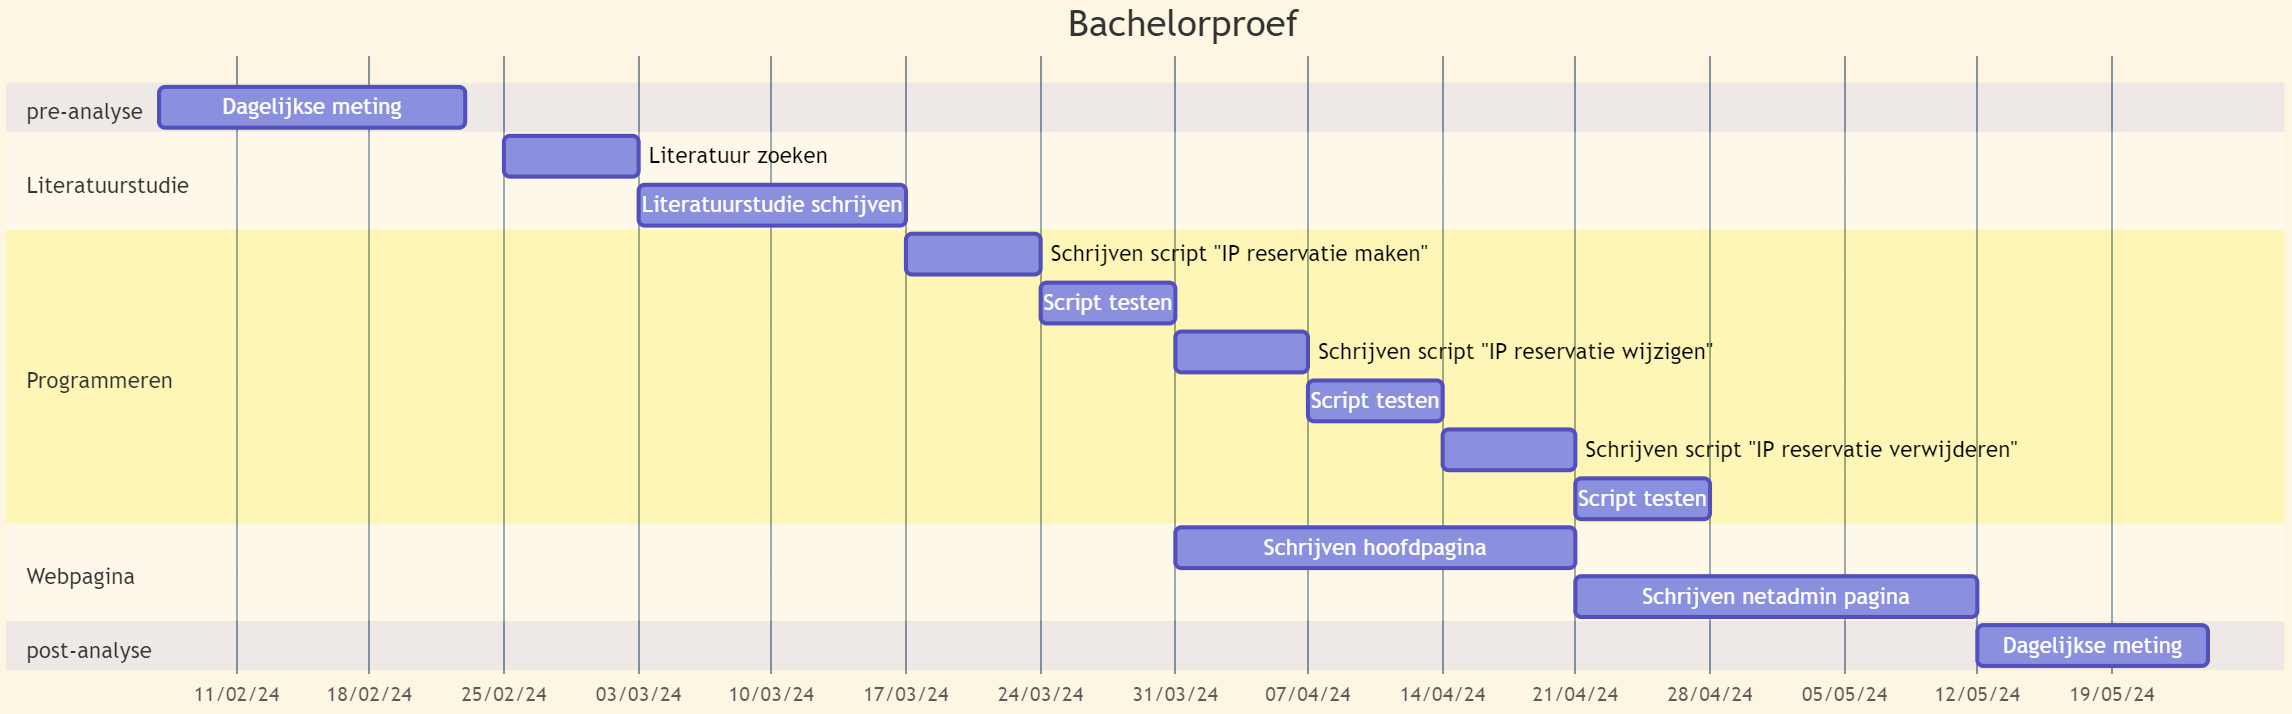
\includegraphics[scale=0.28]{Gantt}
    \caption{Gantt Stappenplan}
    \label{Gantt Stappenplan}
\end{figure}

% Refereren naar de literatuur kan met:
% \autocite{BIBTEXKEY} -> (Auteur, jaartal)
% \textcite{BIBTEXKEY} -> Auteur (jaartal)
% Voorbeeld van een referentie waar de auteursnaam geen onderdeel van de zin is~\autocite{Moore2002}.

\section{Verwachte resultaten}
\label{sec:verwachte-resultaten}
% TODO: (fase 6) beschrijf wat je verwacht uit je onderzoek en waarom (bv. volgens je literatuuronderzoek is softwarepakket A het meest gebruikte en denk je dat het voor deze casus ook het meest geschikt zal zijn). Natuurlijk kan je niet in de toekomst kijken en mag je geen alternatieve mogelijkheden uitsluiten. In de praktijk gebeurt het ook vaak dat een onderzoek tot verrassende resultaten leidt, dat maakt het proces nog interessanter!
De verwachte resultaten omvatten een succesvolle implementatie van de abstractielaag boven de bestaande netwerkbeheer tool, waardoor interacties met EIP mogelijk zijn via Python-scripts. Het intuïtieve webportaal zou een verbeterde gebruikerservaring moeten bieden door middel van geoptimaliseerde API-aanroepen. Verder zou de automatisering van netwerkconfiguraties, \\met name IP-adresallocatie, moeten leiden tot verminderde complexiteit, verbeterde efficiëntie en algemene gebruiksvriendelijkheid in het netwerkbeheerproces.


\section{Discussie, conclusie}
\label{sec:discussie-conclusie}
Dankzij het implementeren van deze webpagina met de onderliggende kunnen medewerkers van Universiteit Gent eenvoudig, consistent, en snel IP reservaties maken, wijzigen en verwijderen. De netwerkbeheerders kunnen al deze wijzigingen dan op hun eigen webpagina controleren, aanpassen en beoordelen.
Na dit onderzoek zullen er nog voldoende mogelijkheden zijn om de webpagina aan te vullen met extra functies tot de mate dat de netwerkbeheerders zelf geen wijzigingen meer moeten doen binnen de IPAM tool zelf.

%------------------------------------------------------------------------------
% Referentielijst
%------------------------------------------------------------------------------
% TODO: (fase 4) de gerefereerde werken moeten in BibTeX-bestand
% bibliografie.bib voorkomen. Gebruik JabRef om je bibliografie bij te
% houden.

\printbibliography[heading=bibintoc]

\end{document}